\chapter{User Guide}\hyperdef{part}{user}{}\label{ch:user}
%----------------------------------
The User Guide is divided into three instruction sets:
\begin{enumerate}
 \item \textbf{Instructions for Simulation Users}.  This instruction-set 
 contains a description of how to modify \ModelDesc\ variables after the 
 simulation has compiled, including an in-depth discussion of the input file; 
 an overview of how to interpret (but not edit) the S\_define file; and a 
 sample of some of the typical variables that may be logged.
 \item \textbf{Instructions for Simulation Developers}.  This instruction-set 
 builds on the previous set, and adds information on the necessary 
 configuration of the \ModelDesc\ within an S\_define file, and the creation of 
 standard run directories.
 \item \textbf{Instructions for Model Developers}.   This instruction-set 
 builds on the previous set, and adds information on the potential for 
 extending the model to perform tasks that are beyond its current abilities.
\end{enumerate}

\section{Instructions for Simulation Users}\label{sec:guide_sim_user}
A simulation user in general does not concern themselves with the \ModelDesc.
The integrators are often created during simulation initialization, which
means that the internal data are not accessible to the Trick logging
mechanisms.
The model works behind the scenes, propagating the states of the simulated
vehicles based on the forces and torques acting on the vehicles.

The simulation's dynamics
manager (see \hypermodelref{DYNMANAGER}) directs the
integration of all dynamic bodies registered with it.
Each dynamic body has its state derivatives computed, based on the forces and
torques acting on it.
The \ModelDesc propagates states according to the state derivatives sent
to it. Properly formulating these state derivatives is one of the jobs of the
\hypermodelref{DYNBODY}.

Two of the factors affecting the accuracy of the propagated state are the
choice of the simulation time step, and the algorithm used to numerically
propagate the state. Every integration algorithm has some optimal
time step for a given problem. Running slower than this optimal step
size reduces accuracy because of limitations inherent in the algorithm.
Running faster than this optimal step size degrades accuracy because the
of limitations inherent in the use of IEEE floating point arithmetic.

For spacecraft simulation that include a model of the flight software, the
operation of the flight software often places an upper bound on the simulation
time step.  The flight software time step is often shorter than the optimal
time-step (viewed from the perspective of accurately propagating state),
resulting in a suboptimal choice for integration rates.  Choosing to run
the simulation at a frequency even greater
than the flight software frequency will further degrade accuracy and
performance, while it is not possible to run more slowly than flight software
requires.  In short, changing the simulation time step is often not an
available option.

There is one marked exception to the above discussion. Ofttimes the behavior
of a failed vehicle must be analyzed. As the flight software is not operating
in these scenarios, the flight software time step is not a constraint.
These scenarios can be run at a frequency slower than the flight software
frequency. Doing so will decrease CPU utilization and may well increase
accuracy.

The appropriate choice of the integration algorithm can
enhance accuracy and performance. The burden of selecting the
appropriate compromise between accuracy and performance falls on the
simulation analyst and integrator. To aid in making that decision, a synopsis
of the techniques available in \JEODid\ is presented in
table~\ref{tab:integ_technique_performance}. The second and third columns
specify the number of calls to the integration and derivative class jobs per
simulation time step. The number of times these functions are called is one of
the key factors that determine the amount of CPU time consumed by a simulation.
The last four columns in the table present the three-sigma error bounds on a
circular orbit simulation integrated with $\omega \Delta t = 0.0562^{\circ}$.
For a 400 km LEO orbit, that corresponds to integrating at 1.15 Hz. These error
bounds are depicted graphically in
Figure~\ref{fig:integ_technique_performance}.

\begin{table}[htp]
\centering
\caption{Integration Technique Performance Characteristics}
\label{tab:integ_technique_performance}
\vspace{1ex}
\begin{tabular}{||l|cccccccc|}
\hline
{\bf Technique} &
\tilt{\bf History length} &
\tilt{\bf Stages per cycle} &
\tilt{\bf Accuracy (order)} &
\tilt{\bf Error, 1 orbit} &
\tilt{\bf Error, 3 orbits} &
\tilt{\bf Error, 10 orbits} &
\tilt{\bf Error, 30 orbits} &
\tilt{\bf Error, 100 orbits} \\ \hline \hline
Euler & 0 & 1 & $O(\Delta t)$ &
  400 km & 3000 & 10000 & 10000 & 20000 km \\
Symplectic Euler & 0 & 1 & $O(\Delta t)$ &
  10 km & 10 & 10 & 10 & 10 km \\
RK2 & 0 & 2 & $O(\Delta t^2)$ &
  0.05 km & 0.2 & 0.5 & 2 & 6 km \\
RK4 & 0 & 4 & $O(\Delta t^4)$ &
  0.002 mm & 0.007 & 0.04 & 0.2 & 0.9 mm \\
ABM4 & 4 & 2 & $O(\Delta t^4)$ &
  0.002 mm & 0.006 & 0.03 & 0.2 & 2 mm \\
Beeman's Algorithm & 1 & 2 & $O(\Delta t^2)$ &
  6 m & 20 & 60 & 200 & 600 m \\
\hline
\end{tabular}
\end{table}

\begin{figure}[htp]
\centering
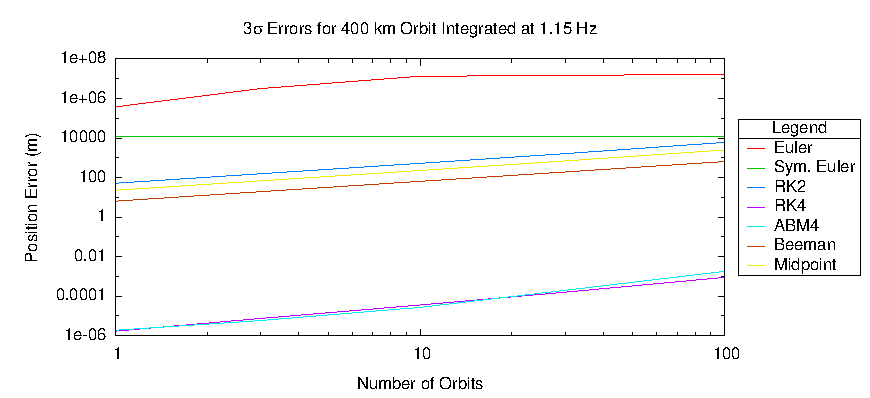
\includegraphics{figures/plot_TranslationTestOrbit_1Hz_monte_err}
\caption{Integration Technique Performance Characteristics}
\label{fig:integ_technique_performance}
\end{figure}


Note that the Euler techniques are quite inaccurate, and their use is
dicouraged.  In particular, use of the basic Euler technique is very strongly
discouraged. It is included with JEOD only because understanding how the basic
Euler technique works is critical for understanding how the more advanced
techniques work.  The symplectic Euler technique may be useful in situations
in which the integration must be
performed at such a high frequency that even a two-stage integrator would be
prohibitively expensive.


\subsection{Changing the Integrator}
The assignment of which integration algorithm will be used is almost always
made at the input file level.  Look for one of the following
specifications:
\begin{verbatim}
 dynamics.manager_init.integ_constructor = trick.<integration-method>()
 dynamics.manager_init.integ_constructor = <sim-object>.<integration-method>
 dynamics.manager_init.jeod_integ_opt = trick.Integration.<integration-method>
 dynamics.manager_init.sim_integ_opt = trick.sim_services.<integration-method>
\end{verbatim}

These are listed in order of preferred practice.

\begin{enumerate}
 \item \textbf{integ\_constructor method with local instantiation}.
 If this method has been used, the
 user will have to look in the S\_define to identify which integrator
 constructors have been included therein.  Look for lines such as

 \verb+##include "utils/integration/include/rk4_integrator_constructor.hh"+

 The integrator can be changed to any of the other integrators for which the
 appropriate header file has been included.  Specifications for
 \verb+<integration-method>+ are:
 \begin{itemize}
  \item ABMIntegratorConstructor
  \item BeemanIntegratorConstructor
  \item EulerIntegratorConstructor
  \item GaussJacksonIntegratorConstructor
  \item RK2IntegratorConstructor
  \item RK4IntegratorConstructor
  \item SymplecticEulerIntegratorConstructor
 \end{itemize}

 Remember to add the () after the specification; this is actually a method
 call to create a new instance of that type of integrator.

 Also be sure to check in the S\_define file to ensure that an instance of the
 IntegratorConstructor has not already been made.  If it has, use option \#2
 (below) instead.

 If the desired integrator is not available, the user may be able to use
 option \#3 (below).


 \item \textbf{integ\_constructor method using S\_define instantiation}.
 If this method has been used,
 the user will have to look in the S\_define to identify which integrator
 constructors have been declared therein (note - these will likely be in the
 simulation object \verb+<sim-object>+).  Any declared constructor can be
 substituted by replacing \verb+<integration-method>+ with the name of
 the instance of another integrator constructor.

 Note that in order for the integrator constructor to be declared, its header
 file must previously be \verb+##include+ in the S\_define, so option \#1
 will, in principle, also work.
 However, if one instance of the integrator
 constructor already exists, another should not be made, so option \#2 is
 preferred \textbf{if} the simulation developer (i.e. the author of the
 S\_define file) has already made such an
 instance.

 If the desired integrator is not available,
 it may be possible to change to option \#3 (below).

 \item \textbf{jeod\_integ\_opt method}. This method can be used with the
 following options for \newline \verb+<integration-method>+:
 \begin{itemize}
  \item Euler
  \item Symplectic Euler
  \item Beeman
  \item RK2
  \item RK4
  \item ABM4
 \end{itemize}
 \item \textbf{sim\_integ\_opt method}.  As a last resort, this method can be
 used with the following options for \verb+<integration-method>+:
 \begin{itemize}
  \item Euler
  \item Euler\_Cromer
  \item Runge\_Kutta\_2
  \item Runge\_Kutta\_4
  \item ABM\_Method
  \end{itemize}
\end{enumerate}

\subsection{Changing the Integration Rate}
The integration rate is typically hard-coded within the simulation.  Look
towards the end of the S\_define file for an entry such as
  \begin{verbatim}
 IntegLoop sim_integ_loop (DYNAMICS) <simulation object list>;
\end{verbatim}
or
\begin{verbatim}
 integrate (DYNAMICS) <simulation object list>;
\end{verbatim}

In either case, the value in parentheses (sometimes a number, sometimes a
parameter) is the integration period.  if a parameter, it will be defined
somewhere in the S\_define, most likely near the top.
\begin{verbatim}
#define DYNAMICS        1.00  // Dynamics interval
\end{verbatim}

There are now two choices for changing the integration rate:
\begin{enumerate}
 \item Change this value; this requires editing the S\_define and recompiling.
 \item Because this value is the simulation-time, and the actual dynamics
 depend on the dynamic-time, it is possible to change (in the input file) the
 actual dynamic-time-step without altering the simulation-time-step by
 altering the rate at which the dynamic-time advances with simulation-time.

 For example,
 \begin{verbatim}
  jeod_time.time_manager.dyn_time.scale_factor = 0.5
 \end{verbatim}
 will make the dynamic-time proceed only half as fast as simulation-time, so a
 simulation-time rate of 1.0 seconds will equate to a dynamic-time rate of 0.5
 seconds.

 Users attempting this change should be familiar with the distinction between
 these two concepts of time. See the \hypermodelref{TIME} for more details.


\end{enumerate}

\subsection{Moving the Integrated Object From One Group to Another}
In rare situation, the simulation may be integrating two different groups of
objects at different rates and.or using different intergators.  It is possible
to switch an object from one group to another, using the
\textit{add\_sim\_object} method.

To identify whether multiple groups are being used, look to the end of the
S\_define for multiple instances of code such as:
\begin{verbatim}
 JeodIntegLoopSimObject <loop_name> (
    <rate>,
    <constructor>,
    <group>,
    <time-manager>,
    <dyn_manager>,
    <gravity_model>,
    <models to be integrated>,
    nullptr);
\end{verbatim}

If this is found, then objects may be moved from one group to another:
\begin{verbatim}
<loop_name>.integ_loop.add_sim_object(<name of object>)
\end{verbatim}
Note - \verb+<loop_name>+ is the name of the group that the object is moving
\textit{to}.


\subsection{Editing the Specifications of the Integrators}
Of the integrators that JEOD provides, only the Gauss-Jackson method has
user-definable specifications.

\subsubsection{Gauss Jackson Parameters}
\label{sec:guide_simuser_gauss_jackson_parameters}
For Gauss-Jackson, the following values can be set:
\begin{itemize}
 \item The order of the integrator.  This defaults to 8, and can be set from 1
 to 16.
 \item The maximum time-step to use on the primer.  This defaults to -1.0;
 indicating that the primer time-step should be the same as the cycle
 time-step and tour time-step.  If the tour time-step is too large for the RK4
 integrator (RK4 serves as the priming integrator, it is used for the first
 few steps) to handle should this value be set.  Set it to a value that is
 appropriate for the limitations of RK4.
 \item Whether or not to perform the convergence test after the correction
 phase.  This defaults to false.
 \item The convergence criterion.  This defaults to $1.0 \times 10^{-9}$.  This
 value is only used if the convergence test is performed.
 \item The maximum number of convergence iterations.  This defaults to 10.  It
 represents the maximum number of times that the state-correction phase can be
 implemented in one integration cycle.  For more precise work, set the
 convergence criterion smaller, and the maximum number of iterations larger.
\end{itemize}

\textbf{Example:}
\begin{verbatim}
 gj_integrator = trick.GaussJacksonIntegratorConstructor()
 gj_integrator.order = 10
 gj_integrator.max_rk4_step= 1.0
 gj_integrator.perform_convergence_test = true
 gj_integrator.convergence_criterion = 1E-10
 gj_integrator.max_corrections_iterations = 15

\end{verbatim}

Note - these values are used in the construction of the integrator.  Once the
constructor has been created, changes to these values will have no effect.
Changes can only be made at the start of the simulation.

The verification simulation \textref{SIM\_GJ\_test}{test:gauss_jackson}
provides a quantitative
illustration of the effect of changing these parameters for a very simple
scenario.


\section{Instructions for Simulation Developers}
Instructions are provided for simulation developers working with the Trick13
simulation engine.  \JEODidx is not compatible with versions of Trick older than 13.0.

\subsection{Populating Integration Groups}\label{sec:user_simdev_groups}
The purpose of integration groups is to
allow the simultaneous integration of models of disparate fidelity
requirements within a single simulation.  In most applications, this tool is
not needed, in which case the default behavior  -- in which there is
only one group -- is assumed.  Each group must define its own integrator
following the steps in
Section~\ref{sec:user_simdev_integrator}.

\subsubsection{Single Group Default Settings}
Without the need for multiple groups, the integration command is
straightforward:

\begin{verbatim}
 IntegLoop sim_integ_loop (DYNAMICS) <simulation object list>;
\end{verbatim}

This command comes at the end of the S\_define.  The argument (e.g. DYNAMICS)
is the integration rate (note - this is based on the simulation time, not the
dynamic time; for the difference, see the Time Model
documentation~\cite{dynenv:TIME}).  Following the argument is a
comma-separated list of all of the simulation objects that need integrating.

An equivalent command is:
\begin{verbatim}
 integrate (DYNAMICS) <simulation object list>;
\end{verbatim}


\subsubsection{Multi-Group Settings}

The prefered method for setting multiple groups is to use the standard module,
\textit{JEOD\_S\_modules/integ\_loop.sm}.  In the S\_define file, include this
file:
\begin{verbatim}
 #include "JEOD_S_modules/integ_loop.sm"
\end{verbatim}

Unlike most of the other sim-modules in the JEOD\_S\_modules directory, this
one
does not create a simulation object, it only defines its contents.

Declare an instance of the DynamicsIntegrationGroup somewhere in the
S\_define, for example in a simulation object called \textit{integ\_object}.  Note that this instance is not going to be used directly, so one instance will suffice for as many groups as are desired.
\begin{verbatim}
 ##include "dynamics/dyn_manager/include/dynamics_integration_group.hh"
 ...
 DynamicsIntegrationGroup group;
\end{verbatim}



At the end of the S\_define, create one instance of the loop object defined in
the integ\_loop file for each intended group.

The structure of this argument is as follows:
\begin{verbatim}
JeodIntegLoopSimObject <name of loop-object> (arguments)
\end{verbatim}

The arguments comprise the following list:
\begin{enumerate}
 \item  The integration-rate.  This is often pre-defined, in which case only
 the name is needed.
 \item  The instance of the desired IntegratorConstructor.  For example, to
 use an Euler integration, declare an instance of EulerIntegratorConstructor
 in integ\_object:
 \begin{verbatim}
 EulerIntegratorConstructor euler_constr;
  \end{verbatim}
  and add the argument \textit{integ\_object.euler\_const}.
  \item An instance of the IntegrationGroup class (e.g.
  \textit{integ\_object.group}).

  \item The TimeManager object for the simulation.  There should be only one,
  if using the standard sim-modules, it will be
  \textit{jeod\_time.time\_manager}.
  \item The Dynamics Manager (DynManager) object.  Again, there should be only
  one in the simulation; if using the standard sim-modules, it will be
  \textit{dynamics.dyn\_manager}.

  \item The gravity manager (GravityManager) object.  Again, there should be only
  one in the simulation; if using the standard sim-modules, it will be
  \textit{env.gravity\_model}.
  \item The address of the first simulation object to be integrated in the
  group.  For example, with a simulation-object called vehicle\_1,
  \textit{\&vehicle\_1}.
  \item Repeat the previous step to add the addresses of as many simulation
  objects as go with this group.
  \item Finish the argument with nullptr to indicate that all objects have been
  entered.
\end{enumerate}

Note that an empty group may be created by specifying no simulation objects.

These examples are taken from
\textit{environment/ephemerides/verif/SIM\_prop\_planet\_T10}.
\begin{verbatim}
 JeodIntegLoopSimObject fast_integ_loop (
    FAST_DYNAMICS,
    integ_constructor.selected_constr, integ_constructor.group,
    jeod_time.time_manager, dynamics.dyn_manager, env.gravity_manager,
    &sun, &jupiter, &saturn, nullptr);


JeodIntegLoopSimObject slow_integ_loop (
    SLOW_DYNAMICS,
    integ_constructor.selected_constr, integ_constructor.group,
    jeod_time.time_manager, dynamics.dyn_manager, env.gravity_manager,
    nullptr);
\end{verbatim}


Once created, objects may be moved from one group to another with the command
\begin{verbatim}
<loop_name>.integ_loop.add_sim_object(<name of object>)
\end{verbatim}

For example, from one of the SIM\_prop\_planet input files

(\textit{environment/ephemerides/verif/SIM\_prop\_planet\_T10/SET\_test/RUN\_switch\_integ/input.py}),
\begin{verbatim}
  slow_integ_loop.integ_loop.add_sim_object(saturn);
\end{verbatim}
It is not necessary to remove an object from its previous integration group.
An object can only belong to one group so is removed automatically.


\subsubsection{Caution on Groups with Different Rates}
While having integration groups with different rates is a valuable tool, it
can
lead to some unfortunate consequences if misused.  The user should be aware
that making a direct comparison of logged values from these two groups may
result in inconsistencies.  Each group will be integrated through its complete
tour before the next group starts.  The objects in the group integrated at
lower frequency will sit with the same state while the higher frequency group
catches up.  Looking at relative states between such entities may lead to
inappropriate conclusions.  When the higher rate is not an integer multiple of
the lower rate (e.g. one at 5Hz and one at 7Hz), the times that the two groups
are providing time-consistent data can be few and far-between.

This is particularly important when switching an object from one group to
another.  When the object switches, its current state is maintained even if it
is invalid at the current time.  For example, suppose some vehicle, was
coasting with an integration period of 10 seconds.  At t=126s, the vehicle is
activated, and now needs integrating at the flight software rate, say 50Hz.
Transitioning immediately to the higher rate group would put the vehicle at
t=126s with the state it had at t=120s (its last integration).  From here
(t=126s), that wrong state will be propagated.






\subsection{Setting the Integration Method}
\label{sec:user_simdev_integrator}

In order to use an integrator, it must be available to the simulation engine
at compilation time.  There are two ways by which this can be done:
\begin{enumerate}
 \item inclusion of the integrator from a standard suite, via an enumerated
 list, or
 \item deliberate declaration of the integrator-constructor in the S\_define.
\end{enumerate}

Having the integrator available without deliberate inclusion may be easier to
implement, but this process has the significant drawback that
the code for that integrator must then be compiled as a part of the simulation
whether it is desired or not.  This time-consuming model is suboptimal, and
while it is supported in the current release, it may be deprecated later.  The
recommended practice, therefore, is to instantiate the integrator-constructors
directly, in either the S\_define or the input file.

To provide backward compatibility, the enumerated list of integrators is still
provided, as is the conversion from the Trick enumerated list.  However, there
are no plans to add new integrators to the list.  Consequently, the only way
to access the Gauss-Jackson method is through the recommended practice of
direct declaration.

Furthermore, when using multiple integration groups, the process for defining
which integrator to use with which group requires that the
integrator-constructor be
available for passing as an argument.  In this case, the
recommended method is required.

The pre-loaded integrators are available via an enumerated list.  The
enumeration value can be accessed from either the JEOD list or specified via
the trick simulation interface method using the comparable
Trick list.

There are three methods available for selecting an integrator, as discussed
below.

\subsubsection {Recommended Practice}

Setting the Dynamics Manager \textit{integ\_constructor} value is the priority
method for defining the integrator.  It is this value that is tested first.

There are two ways to do this:
\begin{enumerate}
 \item \textbf{The easy way:} \newline
 \begin{enumerate}
  \item Include the header file in the S\_define, e.g.
   \begin{verbatim}
   ##include "utils/integration/include/rk4_integrator_constructor.hh"
   \end{verbatim}
   \item then instantiate the Integrator Constructor by assignment in the
     input file, e.g.
   \begin{verbatim}
    dynamics.manager_init.integ_constructor = trick.RK4IntegratorConstructor()
   \end{verbatim}
 \end{enumerate}



 \item \textbf{The more traditional way:} \newline
 \begin{enumerate}
  \item Instantiate an instance of the integrator-constructor in the S\_define.
  \item Point the DynManagerInit value integ\_constructor to the instance of
  the integrator-constructor
 \end{enumerate}

\textbf{Example:}

In the S\_define, create a sim-object called \textit{integ\_sim\_object}, that
includes an instance of a RK4IntegratorConstructor called \textit{rk4}.
\begin{verbatim}
##include "utils/integration/include/rk4_integrator_constructor.hh"
class IntegSimObject: public Trick::SimObject {
...
RK4IntegratorConstructor rk4;
...
}
IntegSimObject integ_sim_object;
\end{verbatim}

In the input file, declare the \textit{integ\_constructor} to be this new
constructor
(note - although the \textit{integ\_constructor} is a pointer, Python can
assign it without having to take the address)

\begin{verbatim}
 dynamics.manager_init.integ_constructor = integ_sim_object.rk4
\end{verbatim}

\end{enumerate}


\subsubsection{Allowable non-optimal practice}

If the integ\_constructor pointer is NULL (i.e. has not been set), then the
next-preferred method is to use the \textit{jeod\_integ\_opt} specification.
The allowable targets for this are the enumerated items in
Table~\ref{tab:user_simdev_jeod_integ}, each prefaced with
\verb+trick.Integration.+~.

\textbf{Example:}
\begin{verbatim}
 dynamics.manager_init.jeod_integ_opt = trick.Integration.RK4
\end{verbatim}

\begin{table}[h!]
\centering
\caption{Integration Technique Enumeration}
\label{tab:user_simdev_jeod_integ}
\vspace{1ex}
\begin{tabular}{||l|c|c|}
\hline
\bf{Integrator} & {\bf Enumeration} & {\bf Trick Equivalent}
\\ \hline \hline
Euler & 1 & Euler \\
Symplectic Euler &2&Euler\_Cromer\\
Beeman &3&N/A\\
RK2 &4&Runge\_Kutta\_2\\
RK4 &5&Runge\_Kutta\_4\\
ABM4 &6&ABM\_Method\\
Gauss-Jackson &N/A&N/A \\
\hline
\end{tabular}
\end{table}

\subsubsection{Deprecated Practice}

It is still possible to declare the method using the Trick enumerated list,
and that practice is still widely used, although it is no longer supprted.
This
method is only followed when both the \textit{integ\_constructor} and
\textit{jeod\_integ\_opt} are not set.  It is
included here to provide simulation developers with information on how to
interpret this command if seen in other simulations.

The \textit{sim\_integ\_opt} value in the dynamics manager initializer can be
set to an element in the Trick integration list.  Note that only those
elements in the Trick integration list that appear in
Table~\ref{tab:user_simdev_jeod_integ} are allowable entries for JEOD
integration.  Each entry must be prefaced with \verb+trick.sim_services+.

\textbf{Example:}
\begin{verbatim}
 dynamics.manager_init.sim_integ_opt = trick.sim_services.Runge_Kutta_4
\end{verbatim}

The four examples above will all produce the same result.



\section{Instructions for Model Developers}

The \ModelDesc is intended to provide a baseline configuration for objects that 
have mass.  It is quite extensible; an example of that extension is in the 
Dynamic Body model, discussed briefly in this document and extensively in the 
Dynamic Body model document (~\cite{dynenv:DYNBODY}).

Authors of an extension will have to pay close attention to the limitations of 
the \ModelDesc, and consider whether the methods provided are suitable for the 
task in the new environment.  For example, when attaching two bodies, the 
\ModelDesc provides all of the functionality associated with positioning the 
mass bodies correctly in the mass tree, with the correct orientation and 
relative positions.  It does not provide any capabilities for modeling the 
changes to the dynamic state, because it knows nothing of any dynamic states.  
Consequently, the Dynamic Body model extension of the \ModelDesc must provide 
its own unique methods for handling state; these are called in addition to the 
generic \ModelDesc methods when two DynBody objects attach.